\section{OBJETIVOS}
  \label{obj}
  \subsection{GENERAL}
    \begin{frame}{OBJETIVOS}
      \framesubtitle{GENERAL}
      Analizar la cinemática, dinámica traslacional y rotacional en el golf.
      \begin{figure}[H]
        \centering
        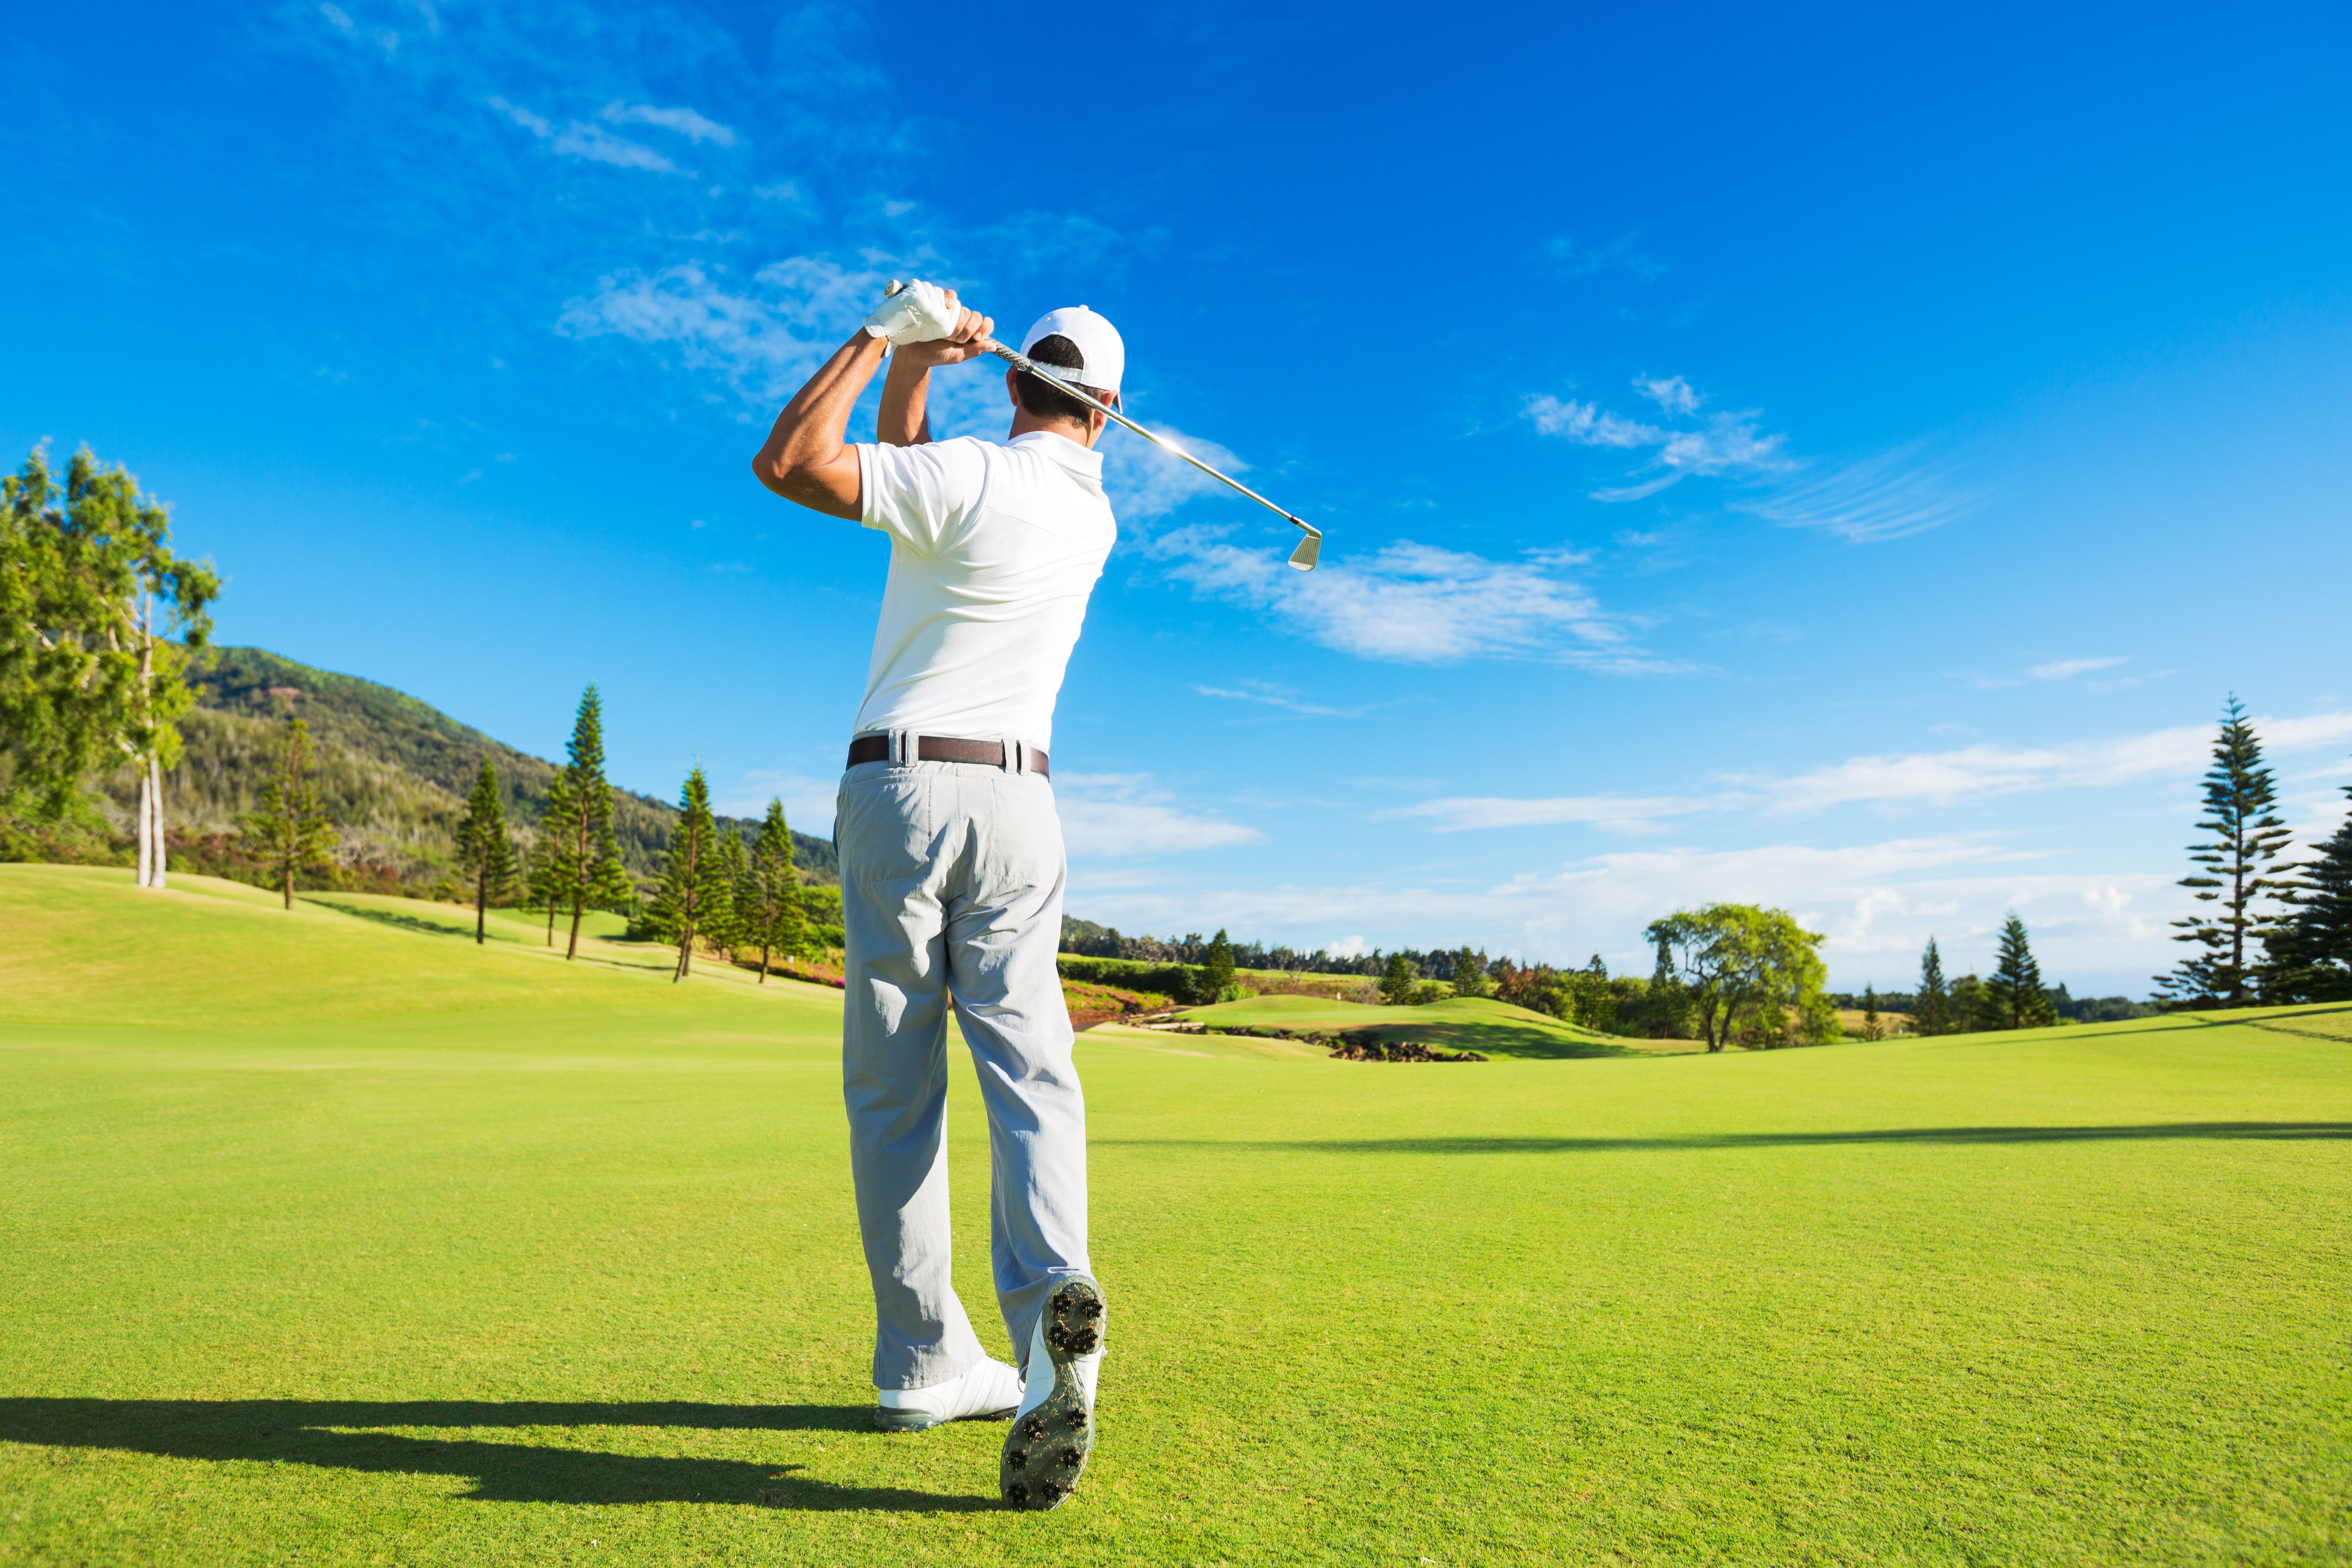
\includegraphics[scale = 0.03]{NiceSwing.jpg}
        \caption{Jugador de golf\footnotemark{}.}
      \end{figure}
      \footnotetext{\bibentry{NiceSwing}.}
    \end{frame}

  \subsection{ESPECÍFICOS}
  \begin{frame}{OBJETIVOS}
    \framesubtitle{ESPECÍFICOS}
    \begin{itemize}
      \item Describir las características recomendadas para los jugadores de golf.
      \item Explicar las funciones e implicaciones físicas de los accesorios presentes en un juego de golf.
      \item Explicar la forma en que los fenómenos físicos afectar la técnica de los jugadores de golf.
      \item Explicar el impacto físico de los implementos utilizados en el golf.
    \end{itemize}
    


  \end{frame}